\documentclass{article}

% Required packages
\usepackage{amssymb}
\usepackage{amsmath}
\usepackage{graphicx}
\usepackage{geometry}
\usepackage{tikz}
\usepackage{array}
\usepackage{booktabs}
\usepackage{enumitem}
\usepackage{listings}
\usepackage{xcolor}
\usepackage{fancyhdr}

% Set page geometry
\geometry{a4paper, margin=1in}

% Configure listings for Python
\lstset{
  language=Python,
  basicstyle=\ttfamily\footnotesize,
  numbers=left,
  numberstyle=\tiny\color{gray},
  frame=single,
  breaklines=true,
  breakatwhitespace=true,
  captionpos=b,
  tabsize=4,
  showspaces=false,
  showstringspaces=false,
  showtabs=false,
  commentstyle=\color{gray}\textit,
  keywordstyle=\color{blue}\bfseries,
  stringstyle=\color{red}
}

% For centering images and tables
\usepackage{float}

\begin{document}

\pagestyle{fancy}
\chead{DSC 255: Machine Learning Fundamentals (Spring 2025)}
\lhead{Homework 2}
\rhead{Randall Rogers}



\textbf{Solution 1 (a)}

\noindent\rule{\textwidth}{0.4pt}\\

\parbox{\textwidth}{The $L_2$ distance is defined as:}\\

$$L_2 = \sqrt{\sum_{i=1}^{n} (x_i - x^{\prime}_i)^2}$$\\

\parbox{\textwidth}{Let, $n = 4$, $x_1 = -1$, $x_2 = 1$, $x_3 = -1$, $x_4 = 1$, $x^{\prime}_1 = 1$, $x^{\prime}_2 = 1$, $x^{\prime}_3 = 1$, $x^{\prime}_4 = 1$.}\\

\parbox{\textwidth}{Use the $L_2$ equation and do the following:}\\

\begin{itemize}
    \item {substitute $n$, expand the summation and subsitute values for $x_1$,..., $x^{\prime}_4$}\\
\end{itemize}

$L_2 = \sqrt{\left((-1 - 1)^2+(1 - 1)^2+(-1 - 1)^2+(1 - 1)^2\right)}$\\

$L_2 = \sqrt{\left((-2)^2+(0)^2+(-2)^2+(0)^2\right)}$\\

$L_2 = \sqrt{\left(4+4\right)}$\\

$L_2 = \sqrt{\left(8\right)}$\\

\parbox{\textwidth}{$\therefore$ the $L_2$ distance between $x$ and $x^{\prime}$ is $\sqrt{8}$.}\\

\noindent\rule{\textwidth}{0.4pt}\\

\newpage

\textbf{Solution 1 (b)}

\noindent\rule{\textwidth}{0.4pt}\\

\parbox{\textwidth}{The $L_1$ distance is defined as:}\\

$$L_1 = \sum_{i=1}^{n} |x_i - x^{\prime}_i|$$\\

\parbox{\textwidth}{Let, $n = 4$, $x_1 = -1$, $x_2 = 1$, $x_3 = -1$, $x_4 = 1$, $x^{\prime}_1 = 1$, $x^{\prime}_2 = 1$, $x^{\prime}_3 = 1$, $x^{\prime}_4 = 1$.}\\

\parbox{\textwidth}{Use the $L_1$ equation and do the following:}\\

\begin{itemize}
    \item {substitute $n$, expand the summation and substitute values for $x_1$,..., $x^{\prime}_4$}\\
\end{itemize}

$L_1 = |(-1 - 1)| + |(1 - 1)| + |(-1 - 1)| + |(1 - 1)|$\\

$L_1 = |(-2)| + |(0)| + |(-2)| + |(0)|$\\

$L_1 = 2 + 0 + 2 + 0$\\

$L_1 = 4$\\

\parbox{\textwidth}{$\therefore$ the $L_1$ distance between $x$ and $x^{\prime}$ is $4$.}\\

\noindent\rule{\textwidth}{0.4pt}\\

\newpage

\textbf{Solution 1 (c)}

\noindent\rule{\textwidth}{0.4pt}\\

\parbox{\textwidth}{The $L_{\infty}$ distance is defined as:}\\

$$L_{\infty} = \max_{i=1,2,...,n} |x_i - x^{\prime}_i|$$\\

\parbox{\textwidth}{Let, $n = 4$, $x_1 = -1$, $x_2 = 1$, $x_3 = -1$, $x_4 = 1$, $x^{\prime}_1 = 1$, $x^{\prime}_2 = 1$, $x^{\prime}_3 = 1$, $x^{\prime}_4 = 1$.}\\

\parbox{\textwidth}{Use the $L_{\infty}$ equation and do the following:}\\

\begin{itemize}
    \item {calculate the absolute differences for each component and find the maximum}\\
\end{itemize}

$L_{\infty} = \max\{|(-1 - 1)|, |(1 - 1)|, |(-1 - 1)|, |(1 - 1)|\}$\\

$L_{\infty} = \max\{|(-2)|, |(0)|, |(-2)|, |(0)|\}$\\

$L_{\infty} = \max\{2, 0, 2, 0\}$\\

$L_{\infty} = 2$\\

\parbox{\textwidth}{$\therefore$ the $L_{\infty}$ distance between $x$ and $x^{\prime}$ is $2$.}\\


\noindent\rule{\textwidth}{0.4pt}

\newpage

\textbf{Solution 2 (a)}

\noindent\rule{\textwidth}{0.4pt}\\

\parbox{\textwidth}{$\|x\|_1$ is defined as:}\\

$$\|x\|_1 = \sum_{i=1}^{n} |x_i|$$\\

\parbox{\textwidth}{Let, $n=3$, $x_1 = 1$, $x_2 = 2$, $x_3 = 3$}\\

\parbox{\textwidth}{Use the $\|x\|_1$ equation and do the following:}\\

\begin{itemize}
    \item {substitute $n$, expand the summation and substitute values for $x_1$, $x_2$, $x_3$}
\end{itemize}

$\|x\|_1 = \sum_{i=1}^{3} |x_i|$\\

$\|x\|_1 = |1| + |2| + |3|$\\

$\|x\|_1 = 6$\\

\parbox{\textwidth}{$\therefore$ $\|x\|_1$ of the point $\begin{bmatrix} 1 \\ 2 \\ 3 \end{bmatrix} \in \mathbb{R}^3$ is $6$.}\\

\noindent\rule{\textwidth}{0.4pt}\\

\newpage

\textbf{Solution 2 (b)}

\noindent\rule{\textwidth}{0.4pt}\\

\parbox{\textwidth}{$\|x\|_2$ is defined as:}\\

$$\|x\|_2 = \sqrt{\sum_{i=1}^{n} x_i^2}$$\\

\parbox{\textwidth}{Let, $n=3$, $x_1 = 1$, $x_2 = 2$, $x_3 = 3$}\\

\parbox{\textwidth}{Use the $\|x\|_2$ equation and do the following:}\\

\begin{itemize}
    \item {substitute $n$, expand the summation and substitute values for $x_1$, $x_2$, $x_3$}
\end{itemize}

$\|x\|_2 = \sqrt{\sum_{i=1}^{3} x_i^2}$\\

$\|x\|_2 = \sqrt{1^2 + 2^2 + 3^2}$\\

$\|x\|_2 = \sqrt{1 + 4 + 9}$\\

$\|x\|_2 = \sqrt{14}$\\

\parbox{\textwidth}{$\therefore$ $\|x\|_2$ of the point $\begin{bmatrix} 1 \\ 2 \\ 3 \end{bmatrix} \in \mathbb{R}^3$  is $\sqrt{14}$.}\\

\noindent\rule{\textwidth}{0.4pt}\\

\newpage

\textbf{Solution 2 (c)}

\noindent\rule{\textwidth}{0.4pt}\\

\parbox{\textwidth}{$\|x\|_{\infty}$ is defined as:}\\

$$\|x\|_{\infty} = \max_{i=1,2,...,n} |x_i|$$\\

\parbox{\textwidth}{Let, $n=3$, $x_1 = 1$, $x_2 = 2$, $x_3 = 3$}\\

\parbox{\textwidth}{Use the $\|x\|_{\infty}$ equation and do the following:}\\

\begin{itemize}
    \item {substitute $n$, find the maximum absolute value among $x_1$, $x_2$, $x_3$}
\end{itemize}

$\|x\|_{\infty} = \max_{i=1,2,3} |x_i|$\\

$\|x\|_{\infty} = \max\{|1|, |2|, |3|\}$\\

$\|x\|_{\infty} = \max\{1, 2, 3\}$\\

$\|x\|_{\infty} = 3$\\

\parbox{\textwidth}{$\therefore$ $\|x\|_{\infty}$ of the point $\begin{bmatrix} 1 \\ 2 \\ 3 \end{bmatrix} \in \mathbb{R}^3$ is $3$.}\\

\noindent\rule{\textwidth}{0.4pt}\\

\newpage

\textbf{Solution 3}

\noindent\rule{\textwidth}{0.4pt}\\

\parbox{\textwidth}{We are given \textit{Table 1}.}

\begin{table}[h]
  \centering
  \begin{tabular}{c|cccc}
    & A & B & C & D \\ \hline
  A & 0 & 2 & 1 & 5 \\
  B & 2 & 0 & 4 & 3 \\
  C & 1 & 4 & 0 & 2 \\
  D & 5 & 3 & 2 & 0 \\
  \end{tabular}
  \caption{Table that specifies a distance function for $\chi$}
  \label{tab:example}
\end{table}

\parbox{\textwidth}{To determine if the given distance function is a metric, it needs to satisfiy the properties of a meteric.}\\

\parbox{\textwidth}{The four properties of a metric are:}\\

\begin{enumerate}
    \item \textbf{Non-negativity}: $d(x,y) \geq 0$ for all $x,y \in \chi$
    \item \textbf{Identity of Indiscernibles}: $d(x,y) = 0$ if and only if $x = y$
    \item \textbf{Symmetry}: $d(x,y) = d(y,x)$ for all $x,y \in \chi$
    \item \textbf{Triangle Inequality}: $d(x,z) \leq d(x,y) + d(y,z)$ for all $x,y,z \in \chi$
\end{enumerate}

\parbox{\textwidth}{Check the first property, Non-negativity.}\\

\parbox{\textwidth}{$0,2,1,5,2,0,4,3,1,4,0,2,5,3,2,0 \geq 0$}\\

\parbox{\textwidth}{Hence, all values are all non-negative and the first property is satisfied.}\\

\parbox{\textwidth}{Now,check the second property, Identity of Indiscernibles.}\\

\parbox{\textwidth}{The points where $x=y$ are the diagonal elements, and it follows that,}\\

\parbox{\textwidth}{these points are $(A,A)$, $(B,B)$, $(C,C)$, and $(D,D)$.}

$$d(A,A) = 0 , d(B,B) = 0 , d(C,C) = 0 , d(D,D) = 0$$

\parbox{\textwidth}{Hence, all diagonal elements are zero and the second property is satisfied.}\\

\parbox{\textwidth}{Next,check the third property, Symmetry.}\\

\parbox{\textwidth}{The symmetry elements are: $(A,B)$ and $(B,A)$; $(A,C)$ and $(C,A)$; $(A,D)$ and $(D,A)$; $(B,C)$ and $(C,B)$; $(B,D)$ and $(D,B)$; $(C,D)$ and $(D,C)$.}\\

\begin{table}[h]
\centering
\begin{tabular}{|c|c|c|}
\hline
$d(x,y)$ & $d(y,x)$ & Distance \\
\hline
$d(A,B)$ & $d(B,A)$  & $2$ \\
$d(A,C)$ & $d(C,A)$  & $1$ \\
$d(A,D)$ & $d(D,A)$  & $5$ \\
$d(B,C)$ & $d(C,B)$  & $4$ \\
$d(B,D)$ & $d(D,B)$  & $3$ \\
$d(C,D)$ & $d(D,C)$  & $2$ \\
\hline
\end{tabular}
\caption{Table that compares distance for $d(x,y)$ and $d(y,x)$ for $\chi$.}
\label{tab:solution}
\end{table}

\parbox{\textwidth}{Hence, all symmetry elements are equal and the third property is satisfied}\\

\begin{itemize}
  \item \parbox{\textwidth}{Note: We could have let $A$ be a matrix that represents \textit{Table 1} and show $A=A^T$}\\
\end{itemize}

\parbox{\textwidth}{Lastly,check the fourth property, Triangle Inequality.}\\

\parbox{\textwidth}{Check if $d(x,z) \leq d(x,y) + d(y,z)$ for all possible combinations of $x$, $y$, and $z$.}\\

\parbox{\textwidth}{Let $x=A$, $y=B$ and $z=C$}\\

\parbox{\textwidth}{Subsitute, $x$, $y$, $z$ into the triangle inequality and evaluate using \textit{Table 2}:}\\

$$d(A,C) \leq d(A,B) + d(B,C) \rightarrow 1 \leq 2 + 4 \rightarrow 1 \leq 6$$

\parbox{\textwidth}{Hence, the Triangle Inequality holds for $x=A$, $y=B$ and $z=C$}\\

\parbox{\textwidth}{Let $x=A$, $y=C$ and $z=D$}\\

\parbox{\textwidth}{Subsitute, $x$, $y$, $z$ into the triangle inequality and evaluate using \textit{Table 2}:}\\

$$d(A,D) \leq d(A,C) + d(C,D) \rightarrow 5 \leq 1 + 2 \rightarrow 5 \nleq 3$$

\parbox{\textwidth}{Hence, for $x=A$, $y=C$ and $z=D$ the Triangle Inequality is not satisfied.}\\

\parbox{\textwidth}{$\therefore$ a distance on the space $\chi$ is not a metric}\\

\noindent\rule{\textwidth}{0.4pt}\\

\newpage

\textbf{Solution 4}

\noindent\rule{\textwidth}{0.4pt}\\

\parbox{\textwidth}{We are given $p$ and $q$ such that:}

$$p =\begin{bmatrix}
    \frac{1}{2} , \frac{1}{4} , \frac{1}{8} , \frac{1}{16} , \frac{1}{16}
\end{bmatrix} , q = \begin{bmatrix}
    \frac{1}{4} , \frac{1}{4} , \frac{1}{6} , \frac{1}{6} , \frac{1}{6}
\end{bmatrix}$$

\parbox{\textwidth}{The Kullback-Leibler (KL) divergence is defined as:}\\

$$K(p,q) = \sum^n_{i=1} p_i \log\left(\frac{p_i}{q_i}\right)$$\\


\parbox{\textwidth}{Let $n = 5$,}\\

\parbox{\textwidth}{$p_1 = \frac{1}{2}$, $p_2 = \frac{1}{4}$, $p_3 = \frac{1}{8}$, $p_4 = \frac{1}{16}$, $p_5 = \frac{1}{16}$}\\

\parbox{\textwidth}{$q_1 = \frac{1}{4}$, $q_2 = \frac{1}{4}$, $q_3 = \frac{1}{6}$, $q_4 = \frac{1}{6}$, $q_5 = \frac{1}{6}$}\\

\begin{itemize}
    \item {substitute $n$, expand the summation and subsitute values for $p_1$,..., $q_5$ in the KL divergence equation}\\
    \item Note: In equation and calculations below $log \equiv log_2$
\end{itemize}

$$K(p,q) = \sum^5_{i=1} p_i \log\left(\frac{p_i}{q_i}\right)$$\\

$K(p,q) = p_1 \log\left(\frac{p_1}{q_1}\right) + p_2 \log\left(\frac{p_2}{q_2}\right) + p_3 \log\left(\frac{p_3}{q_3}\right) + p_4 \log\left(\frac{p_4}{q_4}\right) + p_5 \log\left(\frac{p_5}{q_5}\right)$\\

$K(p,q) = \frac{1}{2} \log\left(\frac{\frac{1}{2}}{\frac{1}{4}}\right) + \frac{1}{4} \log\left(\frac{\frac{1}{4}}{\frac{1}{4}}\right) + \frac{1}{8} \log\left(\frac{\frac{1}{8}}{\frac{1}{6}}\right) + \frac{1}{16} \log\left(\frac{\frac{1}{16}}{\frac{1}{6}}\right) + \frac{1}{16} \log\left(\frac{\frac{1}{16}}{\frac{1}{6}}\right)$\\

$K(p,q) = \frac{1}{2} \log(2) + \frac{1}{4} \log(1) + \frac{1}{8} \log\left(\frac{3}{4}\right) + \frac{1}{16} \log\left(\frac{3}{8}\right) + \frac{1}{16} \log\left(\frac{3}{8}\right)$\\

$K(p,q) \approx 0.2712$\\

\parbox{\textwidth}{$\therefore$ the KL divergence between p and q is approximately $0.082$ }\\

\noindent\rule{\textwidth}{0.4pt}\\

\newpage

\textbf{Solution 5 (a)}

\noindent\rule{\textwidth}{0.4pt}\\

\parbox{\textwidth}{We are attempting to predict a categorical variable (walking, sitting, or running).}\\

\parbox{\textwidth}{$\therefore$ This is best thought as a classification problem.}\\

\noindent\rule{\textwidth}{0.4pt}\\

\newpage

\textbf{Solution 5 (b)}

\noindent\rule{\textwidth}{0.4pt}\\

\parbox{\textwidth}{We are attempting to predict a continuous numerical variable (speed of a car).}\\

\parbox{\textwidth}{$\therefore$ This is best thought as a regression problem.}\\

\noindent\rule{\textwidth}{0.4pt}\\

\newpage

\textbf{Solution 5 (c)}

\noindent\rule{\textwidth}{0.4pt}\\

\parbox{\textwidth}{We are attempting to predict a continuous numerical variable (GPA).}\\

\parbox{\textwidth}{$\therefore$ This is best thought as a regression problem.}\\

\noindent\rule{\textwidth}{0.4pt}\\

\newpage

\textbf{Solution 5 (d)}

\noindent\rule{\textwidth}{0.4pt}\\

\parbox{\textwidth}{We are attempting to predict a categorical variable (pass or not pass).}\\

\parbox{\textwidth}{$\therefore$ This is best thought as a classification problem.}\\

\noindent\rule{\textwidth}{0.4pt}\\

\newpage

\textbf{Solution 6 (a)}

\noindent\rule{\textwidth}{0.4pt}\\

\parbox{\textwidth}{The variance of a random variable $X$ is defined as:}\\

$$\text{Var}(X) = E[(X - \mu)^2] = E[X^2] - (E[X])^2$$

\begin{itemize}
    \item $E[X]$ is the expected value (mean) of $X$
    \item $\mu = E[X]$
\end{itemize}

\parbox{\textwidth}{Since the random variable $X$ takes on values -1 or 1 with equal probability, the probability is $0.50$ or $\frac{1}{2}$.}\\

\parbox{\textwidth}{Let $n = 2$, $x_1 = -1$, $x_2 = 1$, $P(X = x_1) = \frac{1}{2}$, $P(X = x_2) = \frac{1}{2}$.}\\

\parbox{\textwidth}{Calculate the expected value $E[X]$.}\\

$$E[X] = \sum^{n}_{i=1} x_i P(X = x_i)$$

\parbox{\textwidth}{Subsitute $n$, $x_1$, $x_2$, $P(X = x_1), \frac{1}{2}$, $P(X = x_2)$ and expand summation.}\\

$$E[X] = \sum^2_{i=1} x_i \cdot P(X = x_i) = (-1) \cdot \frac{1}{2} + (1) \cdot \frac{1}{2} = -\frac{1}{2} + \frac{1}{2} = 0$$\\

\parbox{\textwidth}{Calculate $E[X^2]$.}\\

\parbox{\textwidth}{Subsitute $n$, $x_1$, $x_2$, $P(X = x_1), \frac{1}{2}$, $P(X = x_2)$ and expand summation.}\\

$$E[X^2] = \sum^2_{i=1} x_i^2 \cdot P(X = x_i) = (-1)^2 \cdot \frac{1}{2} + (1)^2 \cdot \frac{1}{2} = \frac{1}{2} + \frac{1}{2} = 1$$\\

\parbox{\textwidth}{Calculate the variance.}\\

\parbox{\textwidth}{Subsitute $E[X^2]$ and $E[X]$ into the variance equation.}\\

$$\text{Var}(X) = E[X^2] - (E[X])^2 = 1 - (0)^2 = 1 - 0 = 1$$\\

\parbox{\textwidth}{$\therefore$ the variance of $X$ is 1.}\\

\noindent\rule{\textwidth}{0.4pt}\\

\newpage

\textbf{Solution 6 (b)}

\noindent\rule{\textwidth}{0.4pt}\\

\parbox{\textwidth}{The variance of a random variable $X$ is defined as:}\\

$$\text{Var}(X) = E[(X - \mu)^2] = E[X^2] - (E[X])^2$$

\begin{itemize}
    \item $E[X]$ is the expected value (mean) of $X$
    \item $\mu = E[X]$
\end{itemize}

\parbox{\textwidth}{Since the random variable $X$ always takes on the same value, $\exists$ $x$ $\in$ $\mathbb{R}$ such that $P(X=x) =1$.}

\parbox{\textwidth}{Calculate the expected value $E[X]$.}

$$E[X] = \sum^{n}_{i=1} x_i P(X = x_i)$$

\parbox{\textwidth}{Subsitute $n=1$, $x_1=x$, $P(X = x_1) =1$ and expand summation.}\\

$$E[X] = \sum^1_{i=1} x_i \cdot P(X = x_i) = (x) \cdot 1 = x$$

\parbox{\textwidth}{Calculate $E[X^2]$.}

\parbox{\textwidth}{Subsitute $n=1$, $x_1=x$, $P(X = x_1) =1$ and expand summation.}\\

$$E[X^2] = \sum^1_{i=1} x_i^2 \cdot P(X = x_i) = (x)^2 \cdot 1 = x^2$$

\parbox{\textwidth}{Calculate the variance.}\\

\parbox{\textwidth}{Subsitute $E[X^2]$ and $E[X]$ into the variance equation.}\\

$$\text{Var}(X) = E[X^2] - (E[X])^2 = x^2 - x^2 = 0$$

\parbox{\textwidth}{$\therefore$ the variance of $X$ is 0.}

\noindent\rule{\textwidth}{0.4pt}\\

\newpage

\textbf{Solution 6 (c)}

\noindent\rule{\textwidth}{0.4pt}\\

\parbox{\textwidth}{The variance of a random variable $X$ is defined as:}\\

$$\text{Var}(X) = E[(X - \mu)^2] = E[X^2] - (E[X])^2$$

\begin{itemize}
    \item $E[X]$ is the expected value (mean) of $X$
    \item $\mu = E[X]$
\end{itemize}

\parbox{\textwidth}{Let $n = 2$, $x_1 = 1$, $x_2 = 0$, $P(X = x_1) = \frac{1}{4}$, $P(X = x_2) = \frac{3}{4}$.}\\

\parbox{\textwidth}{Calculate the expected value $E[X]$.}\\

$$E[X] = \sum^{n}_{i=1} x_i P(X = x_i)$$

\parbox{\textwidth}{Subsitute $n$, $x_1$, $x_2$, $P(X = x_1)$, $P(X = x_2)$ and expand summation.}\\

$$E[X] = \sum^2_{i=1} x_i \cdot P(X = x_i) = (1) \cdot \frac{1}{4} + (0) \cdot \frac{3}{4} = \frac{1}{4} $$\\

\parbox{\textwidth}{Calculate $E[X^2]$.}\\

\parbox{\textwidth}{Subsitute $n$, $x_1$, $x_2$, $P(X = x_1)$, $P(X = x_2)$ and expand summation.}\\

$$E[X^2] = \sum^2_{i=1} x_i^2 \cdot P(X = x_i) = (1)^2 \cdot \frac{1}{4} + (0)^2 \cdot \frac{3}{4} = \frac{1}{4}$$\\

\parbox{\textwidth}{Calculate the variance.}\\

\parbox{\textwidth}{Subsitute $E[X^2]$ and $E[X]$ into the variance equation.}\\

$$\text{Var}(X) = E[X^2] - (E[X])^2 = \frac{1}{4} - (\frac{1}{4})^2 = \frac{1}{4} - \frac{1}{16} = \frac{3}{16}$$\\

\parbox{\textwidth}{$\therefore$ the variance of $X$ is $\frac{3}{16}$.}\\

\noindent\rule{\textwidth}{0.4pt}\\

\newpage

\textbf{Solution 7 (a)}

\noindent\rule{\textwidth}{0.4pt}\\

\parbox{\textwidth}{We are given \textit{Table 3}.}

\begin{table}[h]
  \centering
  \begin{tabular}{c|ccc}
    $(X\downarrow ,Y \rightarrow)$ & -1 & 0 & 1 \\ \hline
  -1 & 0 & 0 & 1/3 \\
   0 & 0 & 1/3 & 0 \\
   1 & 1/3 & 0 & 0 \\
  \end{tabular}
  \caption{Joint distribution for random variables X and Y.}
  \label{tab:example_fractions}
\end{table}

\parbox{\textwidth}{Covariance for random variables $X$ and $Y$ is defined as:}\\

$$Cov(X,Y) = E[XY] - E[X]E[Y]$$

\parbox{\textwidth}{The expected value of a random variable $X$ is defined as:}\\

$$E[X] = \sum^{n}_{i\in \Omega} x_i P(X)$$

\parbox{\textwidth}{The expected value of a random variable $Y$ is defined as:}\\

$$E[Y] = \sum^{n}_{i\in \Omega} y_i P(Y)$$

\parbox{\textwidth}{The expected value of $XY$  where X and Y are random variables is defined as:}\\

$$E[XY] = \sum_{x} \sum_{y} xy \cdot P(X,Y)$$

\parbox{\textwidth}{Calculate the expected value $E[X]$.}\\

\parbox{\textwidth}{Let $x_1 = -1$, $x_2 = 0$, $x_3 = 1$, and $P(X=-1) = P(X=0) = P(X=1) = \frac{1}{3}$.}\\

$E[X] = (-1) \cdot P(X = -1) + (0) \cdot P(X = 0) + (1) \cdot P(X = 1)$\\

$E[X] = (-1) \cdot \frac{1}{3} + (0) \cdot \frac{1}{3} + (1) \cdot \frac{1}{3}$\\

$E[X] = -\frac{1}{3} + 0 + \frac{1}{3}$\\

$E[X] = 0$\\

\parbox{\textwidth}{Calculate the expected value $E[Y]$.}\\

\parbox{\textwidth}{Let $y_1 = -1$, $y_2 = 0$, $y_3 = 1$, and $P(Y=-1) = P(Y=0) = P(Y=1) = \frac{1}{3}$.}\\

$E[Y] = (-1) \cdot P(Y = -1) + (0) \cdot P(Y = 0) + (1) \cdot P(Y = 1)$\\

$E[Y] = (-1) \cdot \frac{1}{3} + (0) \cdot \frac{1}{3} + (1) \cdot \frac{1}{3}$\\

$E[Y] = -\frac{1}{3} + 0 + \frac{1}{3}$\\

$E[Y] = 0$\\

\parbox{\textwidth}{Calculate the expected value $E[XY]$.}\\

\begin{itemize}
    \item \parbox{\textwidth}{Since we have a diagonal matrix our $E[XY]$ equation becomes the following:}
\end{itemize}

$E[XY] = x_1 y_1\cdot P(X=-1,Y=1) + x_2 y_2\cdot P(X=0,Y=0)+ x_3 y_3\cdot P(X=1,Y=1)$\\

$E[XY] = (-1)(1) \cdot \frac{1}{3} + (0)(0) \cdot \frac{1}{3}+ (1)(-1)\cdot \frac{1}{3}$\\

$E[XY] = -\frac{1}{3} + 0 - \frac{1}{3}$\\

$E[XY] = -\frac{2}{3}$\\

\parbox{\textwidth}{Calculate the covariance.}\\

\parbox{\textwidth}{Subsitute $E[XY]$, $E[X]$ and $E[Y]$ into the covariance equation.}\\

$$Cov(X, Y) = E[XY] - E[X]E[Y] = -\frac{2}{3} - (0)(0) = -\frac{2}{3}$$\\

\parbox{\textwidth}{$\therefore$ the covariance between $X$ and $Y$ is $-\frac{2}{3}$.}\\

\noindent\rule{\textwidth}{0.4pt}\\

\newpage

\textbf{Solution 7 (b)}

\noindent\rule{\textwidth}{0.4pt}\\

\parbox{\textwidth}{Correlation for random variables $X$ and $Y$ is defined as:}\\

$$Corr(X, Y) = \frac{Cov(X, Y)}{\sqrt{Var(X) \cdot Var(Y)}}$$

\parbox{\textwidth}{The variance of a random variable $X$ is defined as:}\\

$$Var(X) = E[X^2] - (E[X])^2$$

\parbox{\textwidth}{The variance of a random variable $Y$ is defined as:}\\

$$Var(Y) = E[Y^2] - (E[Y])^2$$

\begin{itemize}
  \item \parbox{\textwidth}{From \textbf{Solution 7 (a)}, we know that $Cov(X,Y) = -\frac{2}{3}$ and $E[X] = E[Y] = 0$.}\\
\end{itemize}

\parbox{\textwidth}{Calculate $E[X^2]$}\\

$E[X^2] = (-1)^2 \cdot P(X = -1) + (0)^2 \cdot P(X = 0) + (1)^2 \cdot P(X = 1)$\\

$E[X^2] = (-1)^2 \cdot \frac{1}{3} + (0)^2 \cdot \frac{1}{3} + (1)^2 \cdot \frac{1}{3}$\\

$E[X^2] = \frac{1}{3} + 0 + \frac{1}{3}$\\

$E[X^2] = \frac{2}{3}$\\

\parbox{\textwidth}{Calculate $E[Y^2]$}\\

$E[Y^2] = (-1)^2 \cdot P(Y = -1) + (0)^2 \cdot P(Y= 0) + (1)^2 \cdot P(Y= 1)$\\

$E[Y^2] = (-1)^2 \cdot \frac{1}{3} + (0)^2 \cdot \frac{1}{3} + (1)^2 \cdot \frac{1}{3}$\\

$E[Y^2] = \frac{1}{3} + 0 + \frac{1}{3}$\\

$E[Y^2] = \frac{2}{3}$\\


\parbox{\textwidth}{Calculate $Var(X)$.}\\

$Var(X) = E[X^2] - (E[X])^2 = \frac{2}{3} - (0)^2 = \frac{2}{3}$\\

\parbox{\textwidth}{Calculate $Var(Y)$.}\\

$Var(Y) = E[Y^2] - (E[Y])^2 = \frac{2}{3} - (0)^2 = \frac{2}{3}$\\

\parbox{\textwidth}{Calculate $Corr(X,Y)$}\\

\parbox{\textwidth}{Substitute $Cov(X,Y)$, $Var(X)$, and $Var(Y)$ into the correlation equation.}\\

$Corr(X,Y) = \frac{Cov(X,Y)}{\sqrt{Var(X) \cdot Var(Y)}} = \frac{-\frac{2}{3}}{\sqrt{\frac{2}{3} \cdot \frac{2}{3}}} = \frac{-\frac{2}{3}}{\sqrt{\frac{4}{9}}} = \frac{-\frac{2}{3}}{\frac{2}{3}} = -1$\\

\parbox{\textwidth}{$\therefore$ the correlation between $X$ and $Y$ is $-1$.}\\

\noindent\rule{\textwidth}{0.4pt}\\

\newpage

\textbf{Solution 8 (a)}

\noindent\rule{\textwidth}{0.4pt}\\

\parbox{\textwidth}{We are given \textit{Table 4}.}

\begin{table}[h]
  \centering
  \begin{tabular}{c|ccc}
  $(X\downarrow ,Y \rightarrow)$ & -1 & 0 & 1 \\ \hline
  -1 & 1/6 & 0 & 1/6 \\
  0 & 0 & 1/3 & 0 \\
  1 & 1/6 & 0 & 1/6 \\
  \end{tabular}
  \caption{Joint distribution for random variables X and Y.}
  \label{tab:example_fractions}
  \end{table}

\parbox{\textwidth}{Two random variables $X$ and $Y$ are independent if:}\\

$$P(X, Y) = P(X) \cdot P(Y)$$


\parbox{\textwidth}{Calculate probabilities $P(X = -1)$, $P(X = 0)$, and $P(X = 1)$from \textit{Table 4}.}\\

$P(X = -1) = P(X = -1, Y = -1) + P(X = -1, Y = 0) + P(X = -1, Y = 1) = \frac{1}{6} + 0 + \frac{1}{6} = \frac{1}{3}$\\

$P(X = 0) = P(X = 0, Y = -1) + P(X = 0, Y = 0) + P(X = 0, Y = 1) = 0 + \frac{1}{3} + 0 =\frac{1}{3}$\\

$P(X = 1) = P(X = 1, Y = -1) + P(X = 1, Y = 0) + P(X = 1, Y = 1) = \frac{1}{6} + 0 + \frac{1}{6} = \frac{1}{3}$\\


\parbox{\textwidth}{Calculate probabilities $P(Y = -1)$, $P(Y = 0)$, and $P(Y = 1)$from \textit{Table 4}.}\\

$P(Y = -1) = P(X = -1, Y = -1) + P(X = 0, Y = -1) + P(X = 1, Y = -1) =  \frac{1}{6} + 0 + \frac{1}{6} = \frac{1}{3}$\\

$P(Y = 0) = P(X = -1, Y = 0) + P(X = 0, Y = 0) + P(X = 1, Y = 0)= 0 + \frac{1}{3} + 0 =\frac{1}{3}$\\

$P(Y = 1) = P(X = -1, Y = 1) + P(X = 0, Y = 1) + P(X = 1, Y = 1) = \frac{1}{6} + 0 + \frac{1}{6} = \frac{1}{3}$\\


\parbox{\textwidth}{Check if $P(X , Y) = P(X) \cdot P(Y)$ for all combinations:}\\

\parbox{\textwidth}{For $(X = -1, Y = -1)$:}\\

$P(X = -1, Y = -1) = \frac{1}{6}$\\

$P(X = -1) \cdot P(Y = -1) = \frac{1}{3} \cdot \frac{1}{3} = \frac{1}{9}$\\

$$ \frac{1}{6} \neq \frac{1}{9} \rightarrow P(X = -1, Y = -1) \neq P(X = -1) \cdot P(Y = -1)$$\\

\parbox{\textwidth}{$\therefore$ $X$ and $Y$ are not independent.}\\

\noindent\rule{\textwidth}{0.4pt}\\

\newpage

\textbf{Solution 8 (b)}

\noindent\rule{\textwidth}{0.4pt}\\

\parbox{\textwidth}{Two random variables $X$ and $Y$ are uncorrelated if and only if their covariance is zero:}\\

\parbox{\textwidth}{The covariance between $X$ and $Y$ is defined as:}\\

$$Cov(X,Y) = E[XY] - E[X]E[Y]$$

\parbox{\textwidth}{Since,$Cov(X,Y) = 0$ if two random variables are uncorrelated we can check the following expression:}\\

$$E[XY] = E[X]E[Y]$$

\parbox{\textwidth}{Calculate the expected value $E[X]$.}\\

$E[X] = \sum_{x} x \cdot P(X = x)$\\

$E[X] = (-1) \cdot \frac{1}{3} + (0) \cdot \frac{1}{3} + (1) \cdot \frac{1}{3}$\\

$E[X] = -\frac{1}{3} + 0 + \frac{1}{3}$\\

$E[X] = 0$\\

\parbox{\textwidth}{Calculate the expected value $E[Y]$.}\\

$E[Y] = \sum_{y} y \cdot P(Y = y)$\\

$E[Y] = (-1) \cdot \frac{1}{3} + (0) \cdot \frac{1}{3} + (1) \cdot \frac{1}{3}$\\

$E[Y] = -\frac{1}{3} + 0 + \frac{1}{3}$\\

$E[Y] = 0$\\

\parbox{\textwidth}{Calculate the expected value $E[XY]$.}\\

$E[XY] = \sum_{x} \sum_{y} xy \cdot P(X = x, Y = y)$\\

$$E[XY] = (-1)(-1) \cdot \frac{1}{6} + (-1)(0) \cdot 0 + (-1)(1) \cdot \frac{1}{6}+ (0)(-1) \cdot 0 + (0)(0) \cdot \frac{1}{3} + 
(0)(1) \cdot 0+ (1)(-1) \cdot \frac{1}{6} + (1)(0) \cdot 0 + (1)(1) \cdot \frac{1}{6}$$\\

$E[XY] = \frac{1}{6} + 0 + (-\frac{1}{6}) + 0 + 0 + 0 + (-\frac{1}{6}) + 0 + \frac{1}{6}$\\

$E[XY] = \frac{1}{6} - \frac{1}{6} - \frac{1}{6} + \frac{1}{6}$\\

$E[XY] = 0$\\

\parbox{\textwidth}{We have, $E[X]E[Y] = 0$ and $E[XY] = 0$ .}\\

\parbox{\textwidth}{Thus, $E[X]E[Y] = E[XY]$.}\\

\parbox{\textwidth}{$\therefore$ $X$ and $Y$ are uncorrelated.}\\

\noindent\rule{\textwidth}{0.4pt}

\newpage

\textbf{Solution 9 (a)}\\
\noindent\rule{\textwidth}{0.4pt}

\parbox{\textwidth}{Python code for nearest neighbor classifier using $\ell_1$, $\ell_2$, and error rates:}
\begin{center}

\begin{lstlisting}
## import libraries
import numpy as np

## initialize labels for data
data_labels = ['NO','DH','SL']
  
## load data from spine-data.txt and relabel the 7th column (NO:1, DH:1, SL:2)          
data = np.loadtxt('spine-data.txt', converters={6: lambda s: data_labels.index(s)})
  
## split data into features and labels
features = data[:, :-1]
labels = data[:, -1]
  
## split data into training and test sets
features_train = features[:250]
features_test = features[250:]
labels_train = labels[:250]
labels_test = labels[250:]

## define l1 distance function
def l1_distance(x, x_prime):
    l1_dist = np.sum(np.abs(x - x_prime))
    return l1_dist

## define l2 distance function
def l2_distance(x, x_prime):
    l2_dist = np.sqrt(np.sum((x - x_prime) ** 2))
    return l2_dist

## define nn_classifier function
def nn_classifier(features_train, features_test, labels_train,distance_function):
    """
    1. loop through each test point in the features_test list
    2. get the distance between the test point and each training point for every training point
    3. find the index of the training point with the smallest distance
    4. use the index to get the label of the training point
    5. append the label to the predictions list
    6. return the predictions list
    """
    predictions = []
    for test_point in features_test:
        distances = [distance_function(test_point, train_point) for train_point in features_train]
        nearest_neighbor_index = np.argmin(distances)
        predictions.append(labels_train[nearest_neighbor_index])
    return np.array(predictions)

## define error rate function
def get_error_rate(predictions, labels):
    correct = sum(p == l for p, l in zip(predictions, labels))
    accuracy = correct / len(labels)
    return 1 - accuracy

## evaluate l1 distance classifier and get error rate
predictions_l1 = nn_classifier(features_train, features_test, labels_train, l1_distance)
error_rate_l1 = get_error_rate(predictions_l1, labels_test)

## evaluate l2 distance classifier and get error rate
predictions_l2 = nn_classifier(features_train, features_test, labels_train, l2_distance)
error_rate_l2 = get_error_rate(predictions_l2, labels_test)
\end{lstlisting}
    
\end{center}

\parbox{\textwidth}{$\therefore$ the error rates for the two distance functions are: $ER_{\ell_1} = 0.183$ and $ER_{\ell_2} = 0.117$}\\

\noindent\rule{\textwidth}{0.4pt}\\

\newpage

\textbf{Solution 9 (b)}

\noindent\rule{\textwidth}{0.4pt}\\

\parbox{\textwidth}{Python code for confusion matrix for nearest neighbor using $\ell_1$, $\ell_2$, and confusion matrix visualization:}

\begin{itemize}
  \item \parbox{\textwidth}{Note: Utilize functions and variables defined in \textbf{Solution 9 (a)}}
\end{itemize}

\begin{center}

\begin{lstlisting}
## define confusion matrix function
def get_confusion_matrix(predictions, labels):
    cm = confusion_matrix(predictions,labels)
    return cm
  
## visualize confusion matrix function
def plot_confusion_matrix(l1_er, cm1, l2_er, cm2, labels):
    fig, ax = plt.subplots(1,2,figsize=(10, 8),sharey=True)
    ax = ax.flatten()
    sns.heatmap(cm1, annot=True, fmt='d', cmap=sns.color_palette("rocket", as_cmap=True), xticklabels=labels, yticklabels=labels, ax=ax[0])
    ax[0].set_title(f'L1 Distance Confusion Matrix\nError Rate: {l1_er:.3f}')
    sns.heatmap(cm2, annot=True, fmt='d', cmap=sns.color_palette("rocket", as_cmap=True), xticklabels=labels, yticklabels=labels, ax=ax[1])
    ax[1].set_title(f'L2 Distance Confusion Matrix\nError Rate: {l2_er:.3f}')
    ax[0].set_xlabel('Predicted')
    ax[1].set_xlabel('Predicted')
    ax[0].set_ylabel('True')
    plt.tight_layout()
    plt.show()

## get confusion matrix for l1 and l2 distance classifier
cm_l1 = get_confusion_matrix(predictions_l1, labels_test)
cm_l2 = get_confusion_matrix(predictions_l2, labels_test)

## visualize confusion matrix for l1 and l2 distance classifier
plot_confusion_matrix(error_rate_l1, cm_l1, error_rate_l2, cm_l2, data_labels)
\end{lstlisting}
    
\end{center}

\begin{figure}[H]
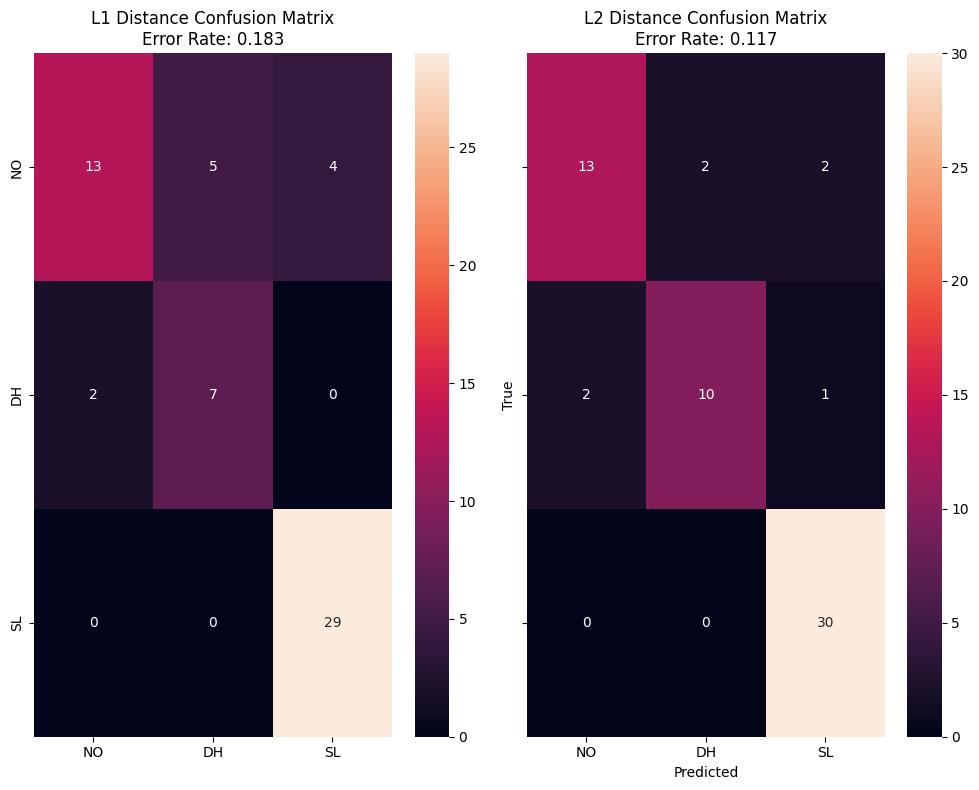
\includegraphics[width=15cm, height=9cm]{q9.png} \\
\caption{Confusion matrix for $\ell_1$ and $\ell_2$ nearest neighbor classifiers.}
\label{fig:image_comparison}
\end{figure} 
      
\noindent\rule{\textwidth}{0.4pt}\\

\newpage

\textbf{Solution 10 (a)}

\noindent\rule{\textwidth}{0.4pt}\\

\parbox{\textwidth}{Python code for reading \textit{wine.DATA}, and splitting data}

\begin{center}

\begin{lstlisting}
## import libraries
import numpy as np
import seaborn as sns
import matplotlib.pyplot as plt
import pandas as pd
import sklearn

## read wine.DATA file
df = pd.read_csv('wine.data', header=None)

## name columns
df.columns = ['Class', 'Alcohol', 'Malic Acid', 'Ash', 'Alcalinity of Ash', 'Magnesium', 'Total Phenols', 'Flavanoids', 'Nonflavanoid Phenols', 'Proanthocyanins', 'Color Intensity', 'Hue', 'OD280/OD315 of Diluted Wines', 'Proline']

## define wine labels
wine_labels = ['Class 1', 'Class 2', 'Class 3']

## split data into features and labels
features = df.iloc[:, 1:].values
labels = df.iloc[:, 0].values

\end{lstlisting}
    
\end{center}

\parbox{\textwidth}{Python code for estimating accuracy and confusion matrix for classifier}
\begin{center}
\begin{lstlisting}

## initalize 1-NN classifier
NN_1 = sklearn.neighbors.KNeighborsClassifier(n_neighbors=1, algorithm='brute', metric='euclidean')
  
## initalize LOOCV
loocv = sklearn.model_selection.LeaveOneOut()
  
## get predictions from cross-validation
predictions = sklearn.model_selection.cross_val_predict(NN_1, features, labels, cv=loocv)
  
## estimate accuracy
accuracy = sklearn.metrics.accuracy_score(labels, predictions)
print(f'Accuracy: {accuracy:.3f}')
## get confusion matrix
cm = sklearn.metrics.confusion_matrix(labels, predictions)
  
## visualize confusion matrix
plt.figure(figsize=(10, 8))
sns.heatmap(cm, annot=True, fmt='d', cmap=sns.color_palette("rocket", as_cmap=True), xticklabels=wine_labels, yticklabels=wine_labels)
plt.title(f'Wine Classification Confusion Matrix\n Accuracy: {accuracy:.3f}')
plt.xlabel('Predicted')
plt.ylabel('True')
plt.tight_layout()
plt.show()

\end{lstlisting}
\end{center}
  
\begin{figure}[H]
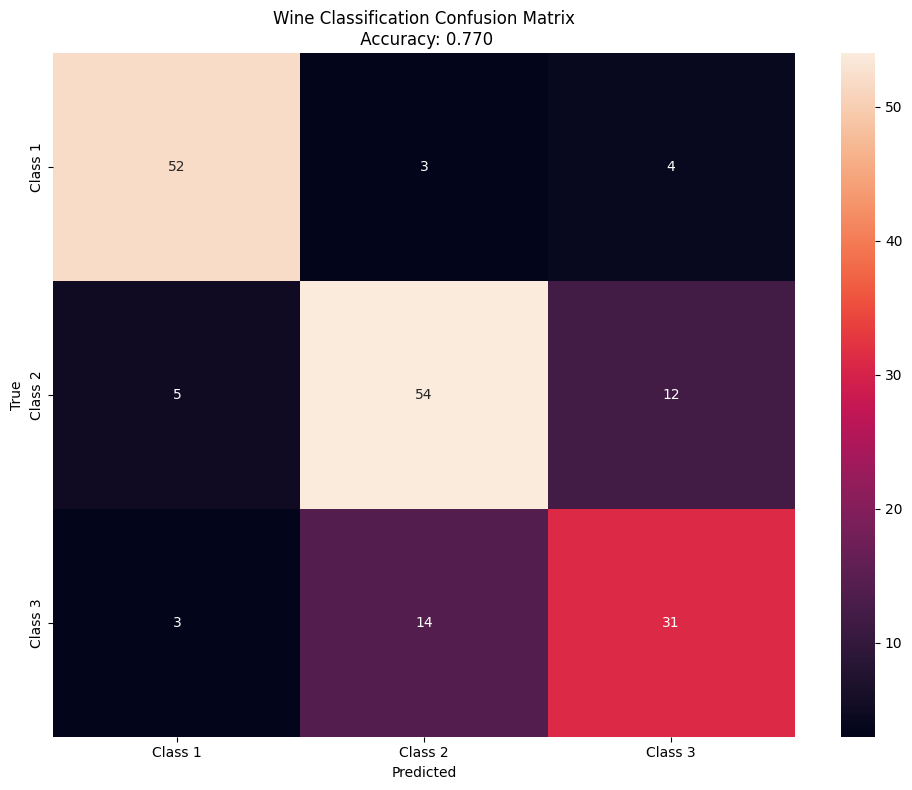
\includegraphics[width=1\textwidth]{q10_a.png} \\
\caption{Estimate of confusion matrix using leave-one-out cross-validation (LOOCV) and 1-NN classification with Euclidean distance.}
\label{fig:image_comparison}
\end{figure} 


\noindent\rule{\textwidth}{0.4pt}\\

\newpage

\textbf{Solution 10 (b)}

\noindent\rule{\textwidth}{0.4pt}\\

\parbox{\textwidth}{Python code for estimating accuracy using k-fold cross-validation and visualization of the estimates}\\

\begin{center}
\begin{lstlisting}
## initialize k values such that we have  20 k's spread out across the range 2 to 100
k_values = np.linspace(2, 100, 20, dtype=int)
  
## initialize accuracy list
accuracies = []
  
## perform k-fold cross-validation for each k
for k in k_values:
    cv = sklearn.model_selection.KFold(n_splits=k, shuffle=True, random_state=42)
    scores = sklearn.model_selection.cross_val_score(NN_1, features, labels, cv=cv)
    accuracies.append(np.mean(scores))
  
## plot results
plt.figure(figsize=(10, 6))
plt.plot(k_values, accuracies, marker='o', linestyle='-')
plt.xlabel('Number of Folds (k)')
plt.ylabel('Accuracy Estimate')
plt.title('Accuracy Estimates for Different Values of k in k-Fold Cross-Validation')
plt.grid(True)
plt.show()
\end{lstlisting}
\end{center}

\begin{figure}[htbp]
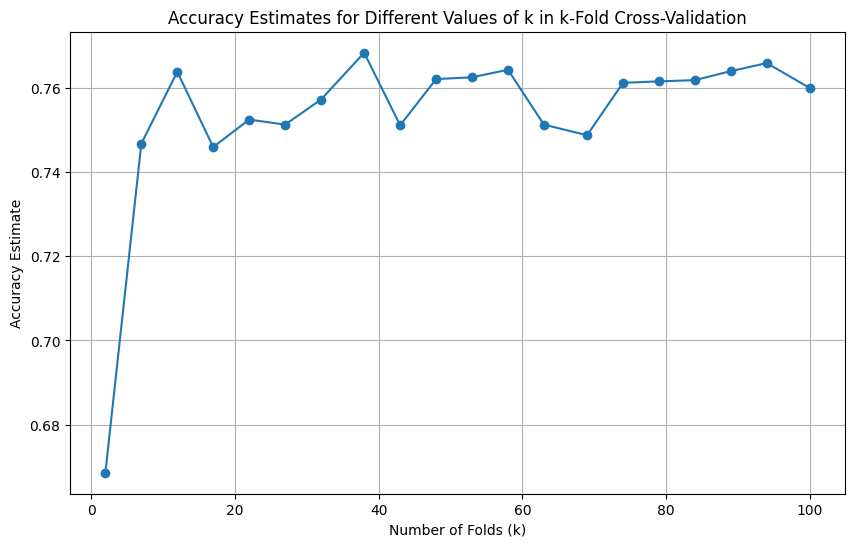
\includegraphics[width=1\textwidth]{q10_b.png} \\
\caption{Estimates of k-fold cross validation accuracies.}
\label{fig:image_comparison}
\end{figure} 

\noindent\rule{\textwidth}{0.4pt}\\

\newpage

\textbf{Solution 10 (c)}

\noindent\rule{\textwidth}{0.4pt}\\

\parbox{\textwidth}{Python code for normalizing data and estimating accuracy and confusion matrix using LOOCV}

\begin{center}

\begin{lstlisting}
## normalize the features
norm_features = sklearn.preprocessing.normalize(features,norm='max')
  
## initalize 1-NN classifier
NN_1_n = sklearn.neighbors.KNeighborsClassifier(n_neighbors=1, algorithm='brute', metric='euclidean')
  
## initalize LOOCV
loocv_n = sklearn.model_selection.LeaveOneOut()
  
## get predictions from cross-validation
predictions_n = sklearn.model_selection.cross_val_predict(NN_1_n, norm_features, labels, cv=loocv_n)
  
## estimate accuracy
accuracy_n = sklearn.metrics.accuracy_score(labels, predictions_n)
print(f'Accuracy: {accuracy:.3f}')
  
## get confusion matrix
cm_n = sklearn.metrics.confusion_matrix(labels, predictions_n)
  
## compare confusion matrices
def compare_confusion_matrix(acc, cm, acc_norm, cm_n, labels):
    fig, ax = plt.subplots(1,2,figsize=(10, 8),sharey=True)
    ax = ax.flatten()
    sns.heatmap(cm, annot=True, fmt='d', cmap=sns.color_palette("rocket", as_cmap=True), xticklabels=labels, yticklabels=labels, ax=ax[0])
    ax[0].set_title(f'Part (a) Confusion Matrix\nAccuracy: {acc:.3f}')
    sns.heatmap(cm_n, annot=True, fmt='d', cmap=sns.color_palette("rocket", as_cmap=True), xticklabels=labels, yticklabels=labels, ax=ax[1])
    ax[1].set_title(f'Confusion Matrix for Normalized Features\nAccuracy: {acc_norm:.3f}')
    ax[0].set_xlabel('Predicted')
    ax[1].set_xlabel('Predicted')
    ax[0].set_ylabel('True')
    plt.tight_layout()
    plt.show()
  
  compare_confusion_matrix(accuracy, cm, accuracy_n, cm_n, wine_labels)
\end{lstlisting}

\end{center}

\begin{figure}[H]

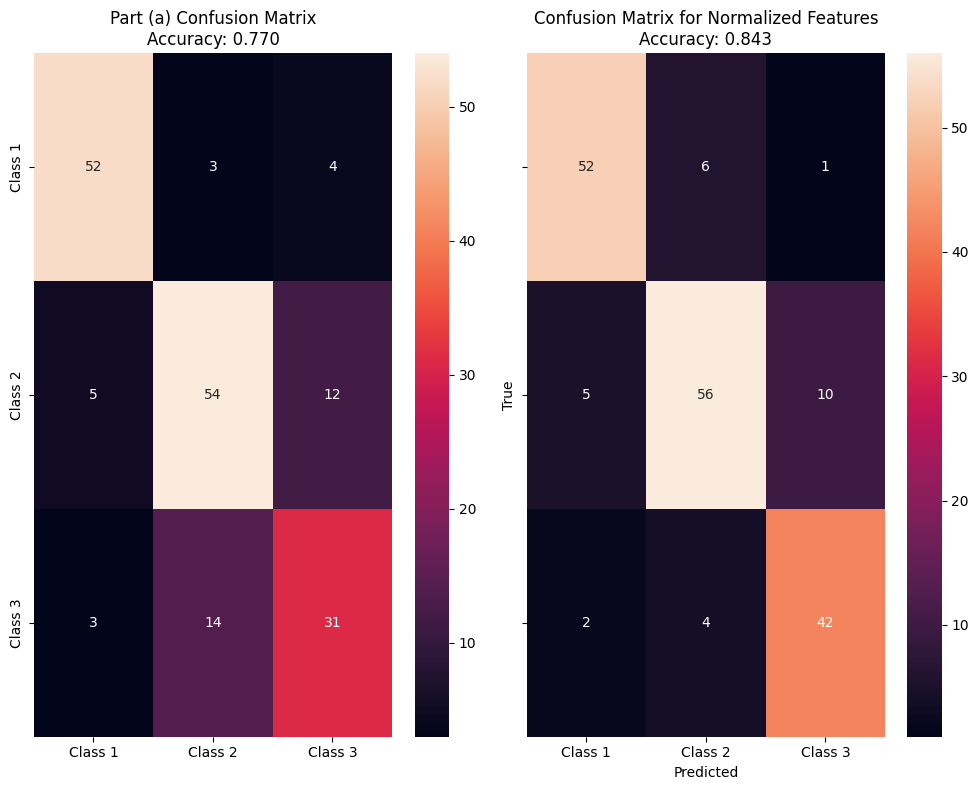
\includegraphics[width=15cm, height=9cm]{q10_c.png} 
\caption{Estimate of confusion matrix for orginal data and normalized data using leave-one-out cross-validation (LOOCV) and 1-NN classification with Euclidean distance.}

\end{figure}

\parbox{\textwidth}{$\therefore$ from \textit{Figure 4} normalizing data improved the performance of the classifier.}\\

\noindent\rule{\textwidth}{0.4pt}\\

\end{document}